% Created by tikzDevice version 0.12.6 on 2024-03-09 08:55:09
% !TEX encoding = UTF-8 Unicode
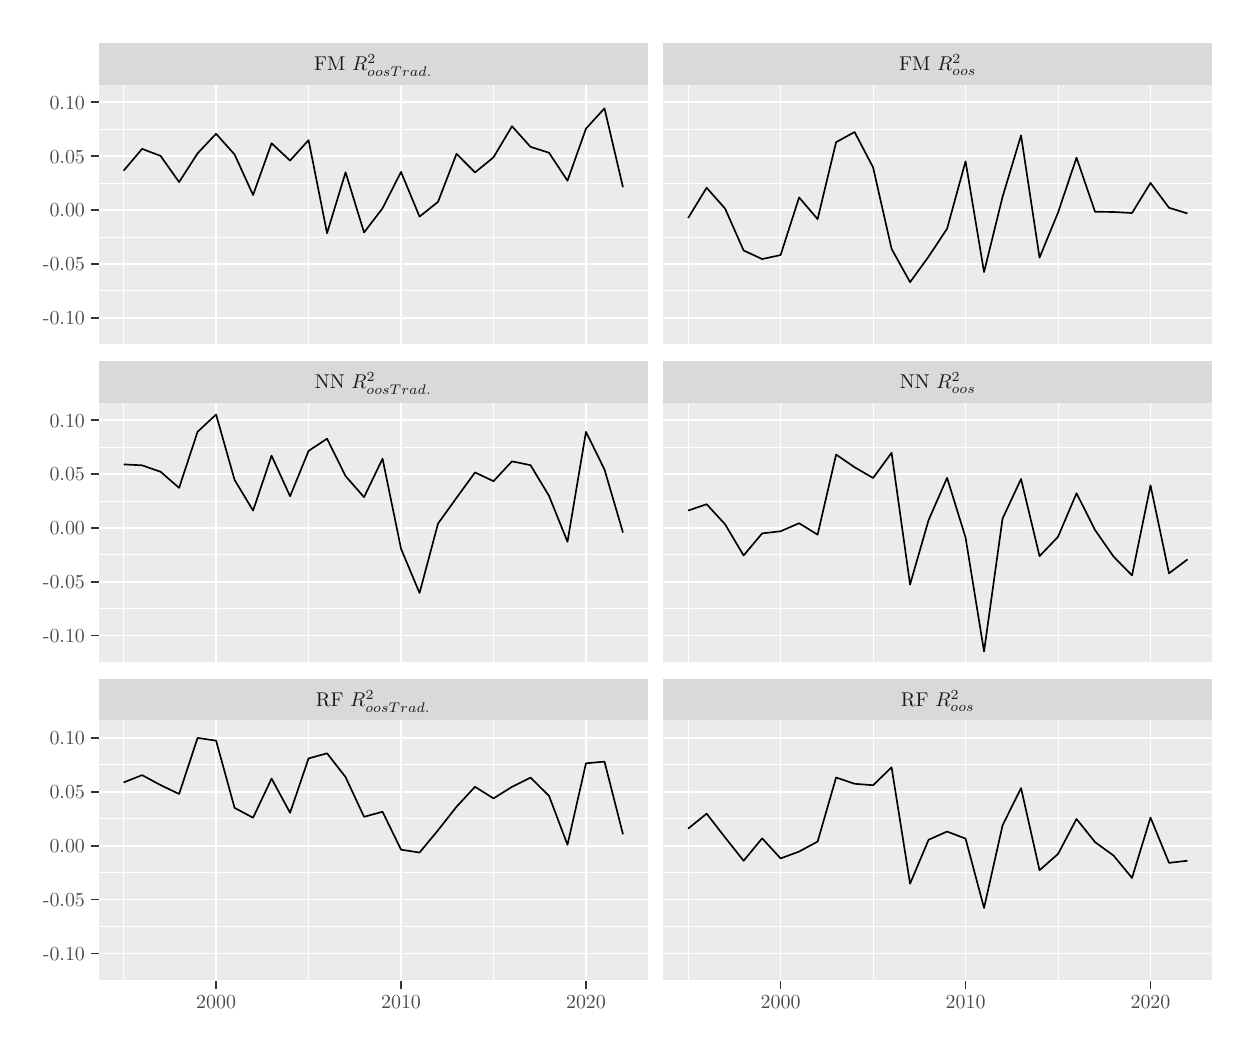
\begin{tikzpicture}[x=1pt,y=1pt]
\definecolor{fillColor}{RGB}{255,255,255}
\path[use as bounding box,fill=fillColor,fill opacity=0.00] (0,0) rectangle (433.62,361.35);
\begin{scope}
\path[clip] (  0.00,  0.00) rectangle (433.62,361.35);
\definecolor{drawColor}{RGB}{255,255,255}
\definecolor{fillColor}{RGB}{255,255,255}

\path[draw=drawColor,line width= 0.6pt,line join=round,line cap=round,fill=fillColor] (  0.00,  0.00) rectangle (433.62,361.35);
\end{scope}
\begin{scope}
\path[clip] ( 25.65,246.50) rectangle (224.13,340.69);
\definecolor{fillColor}{gray}{0.92}

\path[fill=fillColor] ( 25.65,246.50) rectangle (224.13,340.69);
\definecolor{drawColor}{RGB}{255,255,255}

\path[draw=drawColor,line width= 0.3pt,line join=round] ( 25.65,246.80) --
	(224.13,246.80);

\path[draw=drawColor,line width= 0.3pt,line join=round] ( 25.65,266.26) --
	(224.13,266.26);

\path[draw=drawColor,line width= 0.3pt,line join=round] ( 25.65,285.72) --
	(224.13,285.72);

\path[draw=drawColor,line width= 0.3pt,line join=round] ( 25.65,305.18) --
	(224.13,305.18);

\path[draw=drawColor,line width= 0.3pt,line join=round] ( 25.65,324.64) --
	(224.13,324.64);

\path[draw=drawColor,line width= 0.3pt,line join=round] ( 34.67,246.50) --
	( 34.67,340.69);

\path[draw=drawColor,line width= 0.3pt,line join=round] (101.50,246.50) --
	(101.50,340.69);

\path[draw=drawColor,line width= 0.3pt,line join=round] (168.33,246.50) --
	(168.33,340.69);

\path[draw=drawColor,line width= 0.6pt,line join=round] ( 25.65,256.53) --
	(224.13,256.53);

\path[draw=drawColor,line width= 0.6pt,line join=round] ( 25.65,275.99) --
	(224.13,275.99);

\path[draw=drawColor,line width= 0.6pt,line join=round] ( 25.65,295.45) --
	(224.13,295.45);

\path[draw=drawColor,line width= 0.6pt,line join=round] ( 25.65,314.91) --
	(224.13,314.91);

\path[draw=drawColor,line width= 0.6pt,line join=round] ( 25.65,334.37) --
	(224.13,334.37);

\path[draw=drawColor,line width= 0.6pt,line join=round] ( 68.08,246.50) --
	( 68.08,340.69);

\path[draw=drawColor,line width= 0.6pt,line join=round] (134.91,246.50) --
	(134.91,340.69);

\path[draw=drawColor,line width= 0.6pt,line join=round] (201.74,246.50) --
	(201.74,340.69);
\definecolor{drawColor}{RGB}{0,0,0}

\path[draw=drawColor,line width= 0.6pt,line join=round] ( 34.67,309.66) --
	( 41.35,317.56) --
	( 48.03,315.00) --
	( 54.72,305.55) --
	( 61.40,315.94) --
	( 68.08,323.00) --
	( 74.77,315.52) --
	( 81.45,300.88) --
	( 88.13,319.57) --
	( 94.82,313.32) --
	(101.50,320.71) --
	(108.18,287.08) --
	(114.87,309.08) --
	(121.55,287.34) --
	(128.23,296.08) --
	(134.91,309.22) --
	(141.60,293.07) --
	(148.28,298.42) --
	(154.96,315.77) --
	(161.65,309.03) --
	(168.33,314.50) --
	(175.01,325.72) --
	(181.70,318.27) --
	(188.38,316.16) --
	(195.06,306.04) --
	(201.74,324.87) --
	(208.43,332.19) --
	(215.11,303.67);
\end{scope}
\begin{scope}
\path[clip] ( 25.65,131.66) rectangle (224.13,225.84);
\definecolor{fillColor}{gray}{0.92}

\path[fill=fillColor] ( 25.65,131.66) rectangle (224.13,225.84);
\definecolor{drawColor}{RGB}{255,255,255}

\path[draw=drawColor,line width= 0.3pt,line join=round] ( 25.65,131.96) --
	(224.13,131.96);

\path[draw=drawColor,line width= 0.3pt,line join=round] ( 25.65,151.42) --
	(224.13,151.42);

\path[draw=drawColor,line width= 0.3pt,line join=round] ( 25.65,170.88) --
	(224.13,170.88);

\path[draw=drawColor,line width= 0.3pt,line join=round] ( 25.65,190.34) --
	(224.13,190.34);

\path[draw=drawColor,line width= 0.3pt,line join=round] ( 25.65,209.80) --
	(224.13,209.80);

\path[draw=drawColor,line width= 0.3pt,line join=round] ( 34.67,131.66) --
	( 34.67,225.84);

\path[draw=drawColor,line width= 0.3pt,line join=round] (101.50,131.66) --
	(101.50,225.84);

\path[draw=drawColor,line width= 0.3pt,line join=round] (168.33,131.66) --
	(168.33,225.84);

\path[draw=drawColor,line width= 0.6pt,line join=round] ( 25.65,141.69) --
	(224.13,141.69);

\path[draw=drawColor,line width= 0.6pt,line join=round] ( 25.65,161.15) --
	(224.13,161.15);

\path[draw=drawColor,line width= 0.6pt,line join=round] ( 25.65,180.61) --
	(224.13,180.61);

\path[draw=drawColor,line width= 0.6pt,line join=round] ( 25.65,200.07) --
	(224.13,200.07);

\path[draw=drawColor,line width= 0.6pt,line join=round] ( 25.65,219.53) --
	(224.13,219.53);

\path[draw=drawColor,line width= 0.6pt,line join=round] ( 68.08,131.66) --
	( 68.08,225.84);

\path[draw=drawColor,line width= 0.6pt,line join=round] (134.91,131.66) --
	(134.91,225.84);

\path[draw=drawColor,line width= 0.6pt,line join=round] (201.74,131.66) --
	(201.74,225.84);
\definecolor{drawColor}{RGB}{0,0,0}

\path[draw=drawColor,line width= 0.6pt,line join=round] ( 34.67,203.54) --
	( 41.35,203.20) --
	( 48.03,200.87) --
	( 54.72,195.06) --
	( 61.40,215.33) --
	( 68.08,221.56) --
	( 74.77,197.92) --
	( 81.45,186.85) --
	( 88.13,206.69) --
	( 94.82,192.01) --
	(101.50,208.41) --
	(108.18,212.82) --
	(114.87,199.31) --
	(121.55,191.70) --
	(128.23,205.60) --
	(134.91,173.06) --
	(141.60,157.07) --
	(148.28,182.16) --
	(154.96,191.44) --
	(161.65,200.63) --
	(168.33,197.47) --
	(175.01,204.64) --
	(181.70,203.26) --
	(188.38,192.18) --
	(195.06,175.57) --
	(201.74,215.31) --
	(208.43,201.70) --
	(215.11,178.91);
\end{scope}
\begin{scope}
\path[clip] ( 25.65, 16.81) rectangle (224.13,111.00);
\definecolor{fillColor}{gray}{0.92}

\path[fill=fillColor] ( 25.65, 16.81) rectangle (224.13,111.00);
\definecolor{drawColor}{RGB}{255,255,255}

\path[draw=drawColor,line width= 0.3pt,line join=round] ( 25.65, 17.11) --
	(224.13, 17.11);

\path[draw=drawColor,line width= 0.3pt,line join=round] ( 25.65, 36.57) --
	(224.13, 36.57);

\path[draw=drawColor,line width= 0.3pt,line join=round] ( 25.65, 56.03) --
	(224.13, 56.03);

\path[draw=drawColor,line width= 0.3pt,line join=round] ( 25.65, 75.49) --
	(224.13, 75.49);

\path[draw=drawColor,line width= 0.3pt,line join=round] ( 25.65, 94.95) --
	(224.13, 94.95);

\path[draw=drawColor,line width= 0.3pt,line join=round] ( 34.67, 16.81) --
	( 34.67,111.00);

\path[draw=drawColor,line width= 0.3pt,line join=round] (101.50, 16.81) --
	(101.50,111.00);

\path[draw=drawColor,line width= 0.3pt,line join=round] (168.33, 16.81) --
	(168.33,111.00);

\path[draw=drawColor,line width= 0.6pt,line join=round] ( 25.65, 26.84) --
	(224.13, 26.84);

\path[draw=drawColor,line width= 0.6pt,line join=round] ( 25.65, 46.30) --
	(224.13, 46.30);

\path[draw=drawColor,line width= 0.6pt,line join=round] ( 25.65, 65.76) --
	(224.13, 65.76);

\path[draw=drawColor,line width= 0.6pt,line join=round] ( 25.65, 85.22) --
	(224.13, 85.22);

\path[draw=drawColor,line width= 0.6pt,line join=round] ( 25.65,104.68) --
	(224.13,104.68);

\path[draw=drawColor,line width= 0.6pt,line join=round] ( 68.08, 16.81) --
	( 68.08,111.00);

\path[draw=drawColor,line width= 0.6pt,line join=round] (134.91, 16.81) --
	(134.91,111.00);

\path[draw=drawColor,line width= 0.6pt,line join=round] (201.74, 16.81) --
	(201.74,111.00);
\definecolor{drawColor}{RGB}{0,0,0}

\path[draw=drawColor,line width= 0.6pt,line join=round] ( 34.67, 88.60) --
	( 41.35, 91.26) --
	( 48.03, 87.65) --
	( 54.72, 84.45) --
	( 61.40,104.70) --
	( 68.08,103.72) --
	( 74.77, 79.42) --
	( 81.45, 75.86) --
	( 88.13, 90.01) --
	( 94.82, 77.65) --
	(101.50, 97.29) --
	(108.18, 99.14) --
	(114.87, 90.55) --
	(121.55, 76.19) --
	(128.23, 78.03) --
	(134.91, 64.32) --
	(141.60, 63.29) --
	(148.28, 71.33) --
	(154.96, 79.83) --
	(161.65, 87.04) --
	(168.33, 82.84) --
	(175.01, 87.03) --
	(181.70, 90.35) --
	(188.38, 83.78) --
	(195.06, 66.09) --
	(201.74, 95.54) --
	(208.43, 96.13) --
	(215.11, 69.88);
\end{scope}
\begin{scope}
\path[clip] (229.63,246.50) rectangle (428.12,340.69);
\definecolor{fillColor}{gray}{0.92}

\path[fill=fillColor] (229.63,246.50) rectangle (428.12,340.69);
\definecolor{drawColor}{RGB}{255,255,255}

\path[draw=drawColor,line width= 0.3pt,line join=round] (229.63,246.80) --
	(428.12,246.80);

\path[draw=drawColor,line width= 0.3pt,line join=round] (229.63,266.26) --
	(428.12,266.26);

\path[draw=drawColor,line width= 0.3pt,line join=round] (229.63,285.72) --
	(428.12,285.72);

\path[draw=drawColor,line width= 0.3pt,line join=round] (229.63,305.18) --
	(428.12,305.18);

\path[draw=drawColor,line width= 0.3pt,line join=round] (229.63,324.64) --
	(428.12,324.64);

\path[draw=drawColor,line width= 0.3pt,line join=round] (238.66,246.50) --
	(238.66,340.69);

\path[draw=drawColor,line width= 0.3pt,line join=round] (305.49,246.50) --
	(305.49,340.69);

\path[draw=drawColor,line width= 0.3pt,line join=round] (372.32,246.50) --
	(372.32,340.69);

\path[draw=drawColor,line width= 0.6pt,line join=round] (229.63,256.53) --
	(428.12,256.53);

\path[draw=drawColor,line width= 0.6pt,line join=round] (229.63,275.99) --
	(428.12,275.99);

\path[draw=drawColor,line width= 0.6pt,line join=round] (229.63,295.45) --
	(428.12,295.45);

\path[draw=drawColor,line width= 0.6pt,line join=round] (229.63,314.91) --
	(428.12,314.91);

\path[draw=drawColor,line width= 0.6pt,line join=round] (229.63,334.37) --
	(428.12,334.37);

\path[draw=drawColor,line width= 0.6pt,line join=round] (272.07,246.50) --
	(272.07,340.69);

\path[draw=drawColor,line width= 0.6pt,line join=round] (338.90,246.50) --
	(338.90,340.69);

\path[draw=drawColor,line width= 0.6pt,line join=round] (405.73,246.50) --
	(405.73,340.69);
\definecolor{drawColor}{RGB}{0,0,0}

\path[draw=drawColor,line width= 0.6pt,line join=round] (238.66,292.59) --
	(245.34,303.50) --
	(252.02,295.96) --
	(258.70,280.84) --
	(265.39,277.74) --
	(272.07,279.18) --
	(278.75,300.00) --
	(285.44,292.16) --
	(292.12,319.97) --
	(298.80,323.63) --
	(305.49,310.85) --
	(312.17,281.42) --
	(318.85,269.39) --
	(325.54,278.62) --
	(332.22,288.70) --
	(338.90,313.06) --
	(345.58,273.03) --
	(352.27,300.21) --
	(358.95,322.43) --
	(365.63,278.25) --
	(372.32,294.54) --
	(379.00,314.38) --
	(385.68,294.85) --
	(392.37,294.74) --
	(399.05,294.37) --
	(405.73,305.24) --
	(412.41,296.27) --
	(419.10,294.21);
\end{scope}
\begin{scope}
\path[clip] (229.63,131.66) rectangle (428.12,225.84);
\definecolor{fillColor}{gray}{0.92}

\path[fill=fillColor] (229.63,131.66) rectangle (428.12,225.84);
\definecolor{drawColor}{RGB}{255,255,255}

\path[draw=drawColor,line width= 0.3pt,line join=round] (229.63,131.96) --
	(428.12,131.96);

\path[draw=drawColor,line width= 0.3pt,line join=round] (229.63,151.42) --
	(428.12,151.42);

\path[draw=drawColor,line width= 0.3pt,line join=round] (229.63,170.88) --
	(428.12,170.88);

\path[draw=drawColor,line width= 0.3pt,line join=round] (229.63,190.34) --
	(428.12,190.34);

\path[draw=drawColor,line width= 0.3pt,line join=round] (229.63,209.80) --
	(428.12,209.80);

\path[draw=drawColor,line width= 0.3pt,line join=round] (238.66,131.66) --
	(238.66,225.84);

\path[draw=drawColor,line width= 0.3pt,line join=round] (305.49,131.66) --
	(305.49,225.84);

\path[draw=drawColor,line width= 0.3pt,line join=round] (372.32,131.66) --
	(372.32,225.84);

\path[draw=drawColor,line width= 0.6pt,line join=round] (229.63,141.69) --
	(428.12,141.69);

\path[draw=drawColor,line width= 0.6pt,line join=round] (229.63,161.15) --
	(428.12,161.15);

\path[draw=drawColor,line width= 0.6pt,line join=round] (229.63,180.61) --
	(428.12,180.61);

\path[draw=drawColor,line width= 0.6pt,line join=round] (229.63,200.07) --
	(428.12,200.07);

\path[draw=drawColor,line width= 0.6pt,line join=round] (229.63,219.53) --
	(428.12,219.53);

\path[draw=drawColor,line width= 0.6pt,line join=round] (272.07,131.66) --
	(272.07,225.84);

\path[draw=drawColor,line width= 0.6pt,line join=round] (338.90,131.66) --
	(338.90,225.84);

\path[draw=drawColor,line width= 0.6pt,line join=round] (405.73,131.66) --
	(405.73,225.84);
\definecolor{drawColor}{RGB}{0,0,0}

\path[draw=drawColor,line width= 0.6pt,line join=round] (238.66,186.86) --
	(245.34,189.15) --
	(252.02,181.87) --
	(258.70,170.63) --
	(265.39,178.60) --
	(272.07,179.37) --
	(278.75,182.28) --
	(285.44,178.14) --
	(292.12,207.09) --
	(298.80,202.51) --
	(305.49,198.62) --
	(312.17,207.74) --
	(318.85,160.15) --
	(325.54,183.41) --
	(332.22,198.68) --
	(338.90,177.12) --
	(345.58,135.94) --
	(352.27,183.95) --
	(358.95,198.27) --
	(365.63,170.38) --
	(372.32,177.39) --
	(379.00,193.11) --
	(385.68,179.84) --
	(392.37,170.23) --
	(399.05,163.42) --
	(405.73,195.96) --
	(412.41,164.18) --
	(419.10,169.21);
\end{scope}
\begin{scope}
\path[clip] (229.63, 16.81) rectangle (428.12,111.00);
\definecolor{fillColor}{gray}{0.92}

\path[fill=fillColor] (229.63, 16.81) rectangle (428.12,111.00);
\definecolor{drawColor}{RGB}{255,255,255}

\path[draw=drawColor,line width= 0.3pt,line join=round] (229.63, 17.11) --
	(428.12, 17.11);

\path[draw=drawColor,line width= 0.3pt,line join=round] (229.63, 36.57) --
	(428.12, 36.57);

\path[draw=drawColor,line width= 0.3pt,line join=round] (229.63, 56.03) --
	(428.12, 56.03);

\path[draw=drawColor,line width= 0.3pt,line join=round] (229.63, 75.49) --
	(428.12, 75.49);

\path[draw=drawColor,line width= 0.3pt,line join=round] (229.63, 94.95) --
	(428.12, 94.95);

\path[draw=drawColor,line width= 0.3pt,line join=round] (238.66, 16.81) --
	(238.66,111.00);

\path[draw=drawColor,line width= 0.3pt,line join=round] (305.49, 16.81) --
	(305.49,111.00);

\path[draw=drawColor,line width= 0.3pt,line join=round] (372.32, 16.81) --
	(372.32,111.00);

\path[draw=drawColor,line width= 0.6pt,line join=round] (229.63, 26.84) --
	(428.12, 26.84);

\path[draw=drawColor,line width= 0.6pt,line join=round] (229.63, 46.30) --
	(428.12, 46.30);

\path[draw=drawColor,line width= 0.6pt,line join=round] (229.63, 65.76) --
	(428.12, 65.76);

\path[draw=drawColor,line width= 0.6pt,line join=round] (229.63, 85.22) --
	(428.12, 85.22);

\path[draw=drawColor,line width= 0.6pt,line join=round] (229.63,104.68) --
	(428.12,104.68);

\path[draw=drawColor,line width= 0.6pt,line join=round] (272.07, 16.81) --
	(272.07,111.00);

\path[draw=drawColor,line width= 0.6pt,line join=round] (338.90, 16.81) --
	(338.90,111.00);

\path[draw=drawColor,line width= 0.6pt,line join=round] (405.73, 16.81) --
	(405.73,111.00);
\definecolor{drawColor}{RGB}{0,0,0}

\path[draw=drawColor,line width= 0.6pt,line join=round] (238.66, 71.92) --
	(245.34, 77.33) --
	(252.02, 68.72) --
	(258.70, 60.30) --
	(265.39, 68.41) --
	(272.07, 61.16) --
	(278.75, 63.64) --
	(285.44, 67.24) --
	(292.12, 90.40) --
	(298.80, 88.13) --
	(305.49, 87.60) --
	(312.17, 94.08) --
	(318.85, 52.04) --
	(325.54, 67.89) --
	(332.22, 70.87) --
	(338.90, 68.32) --
	(345.58, 43.24) --
	(352.27, 73.10) --
	(358.95, 86.60) --
	(365.63, 56.89) --
	(372.32, 62.78) --
	(379.00, 75.41) --
	(385.68, 67.05) --
	(392.37, 62.20) --
	(399.05, 54.10) --
	(405.73, 75.93) --
	(412.41, 59.55) --
	(419.10, 60.33);
\end{scope}
\begin{scope}
\path[clip] ( 25.65,111.00) rectangle (224.13,126.16);
\definecolor{fillColor}{gray}{0.85}

\path[fill=fillColor] ( 25.65,111.00) rectangle (224.13,126.16);
\definecolor{drawColor}{gray}{0.10}

\node[text=drawColor,anchor=base,inner sep=0pt, outer sep=0pt, scale=  0.72] at (124.89,116.10) {RF $R^2_{oos  Trad.}$};
\end{scope}
\begin{scope}
\path[clip] (229.63,111.00) rectangle (428.12,126.16);
\definecolor{fillColor}{gray}{0.85}

\path[fill=fillColor] (229.63,111.00) rectangle (428.12,126.16);
\definecolor{drawColor}{gray}{0.10}

\node[text=drawColor,anchor=base,inner sep=0pt, outer sep=0pt, scale=  0.72] at (328.88,116.10) {RF $R^2_{oos}$};
\end{scope}
\begin{scope}
\path[clip] ( 25.65,225.84) rectangle (224.13,241.00);
\definecolor{fillColor}{gray}{0.85}

\path[fill=fillColor] ( 25.65,225.84) rectangle (224.13,241.00);
\definecolor{drawColor}{gray}{0.10}

\node[text=drawColor,anchor=base,inner sep=0pt, outer sep=0pt, scale=  0.72] at (124.89,230.94) {NN $R^2_{oos  Trad.}$};
\end{scope}
\begin{scope}
\path[clip] (229.63,225.84) rectangle (428.12,241.00);
\definecolor{fillColor}{gray}{0.85}

\path[fill=fillColor] (229.63,225.84) rectangle (428.12,241.00);
\definecolor{drawColor}{gray}{0.10}

\node[text=drawColor,anchor=base,inner sep=0pt, outer sep=0pt, scale=  0.72] at (328.88,230.94) {NN $R^2_{oos}$};
\end{scope}
\begin{scope}
\path[clip] ( 25.65,340.69) rectangle (224.13,355.85);
\definecolor{fillColor}{gray}{0.85}

\path[fill=fillColor] ( 25.65,340.69) rectangle (224.13,355.85);
\definecolor{drawColor}{gray}{0.10}

\node[text=drawColor,anchor=base,inner sep=0pt, outer sep=0pt, scale=  0.72] at (124.89,345.79) {FM $R^2_{oos  Trad.}$};
\end{scope}
\begin{scope}
\path[clip] (229.63,340.69) rectangle (428.12,355.85);
\definecolor{fillColor}{gray}{0.85}

\path[fill=fillColor] (229.63,340.69) rectangle (428.12,355.85);
\definecolor{drawColor}{gray}{0.10}

\node[text=drawColor,anchor=base,inner sep=0pt, outer sep=0pt, scale=  0.72] at (328.88,345.79) {FM $R^2_{oos}$};
\end{scope}
\begin{scope}
\path[clip] (  0.00,  0.00) rectangle (433.62,361.35);
\definecolor{drawColor}{gray}{0.20}

\path[draw=drawColor,line width= 0.6pt,line join=round] ( 68.08, 14.06) --
	( 68.08, 16.81);

\path[draw=drawColor,line width= 0.6pt,line join=round] (134.91, 14.06) --
	(134.91, 16.81);

\path[draw=drawColor,line width= 0.6pt,line join=round] (201.74, 14.06) --
	(201.74, 16.81);
\end{scope}
\begin{scope}
\path[clip] (  0.00,  0.00) rectangle (433.62,361.35);
\definecolor{drawColor}{gray}{0.30}

\node[text=drawColor,anchor=base,inner sep=0pt, outer sep=0pt, scale=  0.72] at ( 68.08,  6.90) {2000};

\node[text=drawColor,anchor=base,inner sep=0pt, outer sep=0pt, scale=  0.72] at (134.91,  6.90) {2010};

\node[text=drawColor,anchor=base,inner sep=0pt, outer sep=0pt, scale=  0.72] at (201.74,  6.90) {2020};
\end{scope}
\begin{scope}
\path[clip] (  0.00,  0.00) rectangle (433.62,361.35);
\definecolor{drawColor}{gray}{0.20}

\path[draw=drawColor,line width= 0.6pt,line join=round] (272.07, 14.06) --
	(272.07, 16.81);

\path[draw=drawColor,line width= 0.6pt,line join=round] (338.90, 14.06) --
	(338.90, 16.81);

\path[draw=drawColor,line width= 0.6pt,line join=round] (405.73, 14.06) --
	(405.73, 16.81);
\end{scope}
\begin{scope}
\path[clip] (  0.00,  0.00) rectangle (433.62,361.35);
\definecolor{drawColor}{gray}{0.30}

\node[text=drawColor,anchor=base,inner sep=0pt, outer sep=0pt, scale=  0.72] at (272.07,  6.90) {2000};

\node[text=drawColor,anchor=base,inner sep=0pt, outer sep=0pt, scale=  0.72] at (338.90,  6.90) {2010};

\node[text=drawColor,anchor=base,inner sep=0pt, outer sep=0pt, scale=  0.72] at (405.73,  6.90) {2020};
\end{scope}
\begin{scope}
\path[clip] (  0.00,  0.00) rectangle (433.62,361.35);
\definecolor{drawColor}{gray}{0.30}

\node[text=drawColor,anchor=base east,inner sep=0pt, outer sep=0pt, scale=  0.72] at ( 20.70,254.05) {-0.10};

\node[text=drawColor,anchor=base east,inner sep=0pt, outer sep=0pt, scale=  0.72] at ( 20.70,273.51) {-0.05};

\node[text=drawColor,anchor=base east,inner sep=0pt, outer sep=0pt, scale=  0.72] at ( 20.70,292.97) {0.00};

\node[text=drawColor,anchor=base east,inner sep=0pt, outer sep=0pt, scale=  0.72] at ( 20.70,312.43) {0.05};

\node[text=drawColor,anchor=base east,inner sep=0pt, outer sep=0pt, scale=  0.72] at ( 20.70,331.89) {0.10};
\end{scope}
\begin{scope}
\path[clip] (  0.00,  0.00) rectangle (433.62,361.35);
\definecolor{drawColor}{gray}{0.20}

\path[draw=drawColor,line width= 0.6pt,line join=round] ( 22.90,256.53) --
	( 25.65,256.53);

\path[draw=drawColor,line width= 0.6pt,line join=round] ( 22.90,275.99) --
	( 25.65,275.99);

\path[draw=drawColor,line width= 0.6pt,line join=round] ( 22.90,295.45) --
	( 25.65,295.45);

\path[draw=drawColor,line width= 0.6pt,line join=round] ( 22.90,314.91) --
	( 25.65,314.91);

\path[draw=drawColor,line width= 0.6pt,line join=round] ( 22.90,334.37) --
	( 25.65,334.37);
\end{scope}
\begin{scope}
\path[clip] (  0.00,  0.00) rectangle (433.62,361.35);
\definecolor{drawColor}{gray}{0.30}

\node[text=drawColor,anchor=base east,inner sep=0pt, outer sep=0pt, scale=  0.72] at ( 20.70,139.21) {-0.10};

\node[text=drawColor,anchor=base east,inner sep=0pt, outer sep=0pt, scale=  0.72] at ( 20.70,158.67) {-0.05};

\node[text=drawColor,anchor=base east,inner sep=0pt, outer sep=0pt, scale=  0.72] at ( 20.70,178.13) {0.00};

\node[text=drawColor,anchor=base east,inner sep=0pt, outer sep=0pt, scale=  0.72] at ( 20.70,197.59) {0.05};

\node[text=drawColor,anchor=base east,inner sep=0pt, outer sep=0pt, scale=  0.72] at ( 20.70,217.05) {0.10};
\end{scope}
\begin{scope}
\path[clip] (  0.00,  0.00) rectangle (433.62,361.35);
\definecolor{drawColor}{gray}{0.20}

\path[draw=drawColor,line width= 0.6pt,line join=round] ( 22.90,141.69) --
	( 25.65,141.69);

\path[draw=drawColor,line width= 0.6pt,line join=round] ( 22.90,161.15) --
	( 25.65,161.15);

\path[draw=drawColor,line width= 0.6pt,line join=round] ( 22.90,180.61) --
	( 25.65,180.61);

\path[draw=drawColor,line width= 0.6pt,line join=round] ( 22.90,200.07) --
	( 25.65,200.07);

\path[draw=drawColor,line width= 0.6pt,line join=round] ( 22.90,219.53) --
	( 25.65,219.53);
\end{scope}
\begin{scope}
\path[clip] (  0.00,  0.00) rectangle (433.62,361.35);
\definecolor{drawColor}{gray}{0.30}

\node[text=drawColor,anchor=base east,inner sep=0pt, outer sep=0pt, scale=  0.72] at ( 20.70, 24.36) {-0.10};

\node[text=drawColor,anchor=base east,inner sep=0pt, outer sep=0pt, scale=  0.72] at ( 20.70, 43.82) {-0.05};

\node[text=drawColor,anchor=base east,inner sep=0pt, outer sep=0pt, scale=  0.72] at ( 20.70, 63.28) {0.00};

\node[text=drawColor,anchor=base east,inner sep=0pt, outer sep=0pt, scale=  0.72] at ( 20.70, 82.74) {0.05};

\node[text=drawColor,anchor=base east,inner sep=0pt, outer sep=0pt, scale=  0.72] at ( 20.70,102.20) {0.10};
\end{scope}
\begin{scope}
\path[clip] (  0.00,  0.00) rectangle (433.62,361.35);
\definecolor{drawColor}{gray}{0.20}

\path[draw=drawColor,line width= 0.6pt,line join=round] ( 22.90, 26.84) --
	( 25.65, 26.84);

\path[draw=drawColor,line width= 0.6pt,line join=round] ( 22.90, 46.30) --
	( 25.65, 46.30);

\path[draw=drawColor,line width= 0.6pt,line join=round] ( 22.90, 65.76) --
	( 25.65, 65.76);

\path[draw=drawColor,line width= 0.6pt,line join=round] ( 22.90, 85.22) --
	( 25.65, 85.22);

\path[draw=drawColor,line width= 0.6pt,line join=round] ( 22.90,104.68) --
	( 25.65,104.68);
\end{scope}
\end{tikzpicture}
